%# -*- coding: utf-8-unix -*-
%%==================================================
%% chapter02.tex for SJTU Master Thesis
%% based on CASthesis
%% modified by wei.jianwen@gmail.com
%% Encoding: UTF-8
%%==================================================

\chapter{实验}
\label{chap:example}
在本章中,我们通过实验来比较CAH(竞争感知的混合放置框架)、CWS(Compact With Shift)、EE(Enhanced Even)、Compact及Even五种线程放置策略,对C-MCS锁的性能(吞吐率)和长期公平性方面的影响,其中CWS和EE是CAH框架中的两个基本线程放置策略,Even是AHMCS\cite{chabbi2016contention}中采用的平均线程放置策略,而Compact是HMCS\cite{chabbi2015high}和HMCS-T\cite{chabbi2017efficient}等大多数基于队列的层级锁中采用的紧凑线程放置策略。我们使用变异系数(CV, coefficient of variation)及劳伦茨曲线\cite{gini1912variabilita}来衡量和展示长期公平性。在本文的实验中,变异系数描述了参与锁竞争的线程集合中每个线程的拿锁次数分布特征,这个系数越接近0表示长期公平性越好,越接近1则表示长期公平性越差。

实验分别在stress\_one和Memcached两个benchmark上进行,其中stress\_one是一个microbenchmark,而Memcached则是现实世界中广泛使用的有实际负载的应用。通过在stress\_one的实验可以让我们把握不同线程放置策略对锁的相关特征的趋向性的影响,而在Memcached上的实验则可以验证其在现实应用中的效果。为了验证CAH在负载/竞争动态变化时的有效性,我们对stress\_one进行了修改,使其中的pause time每200ms在输入的pause time的上下某个范围内随机波动,然后分别统计在stress\_one运行的10s内的吞吐率和各个线程的吞吐率分布,进而比较不同线程放置策略下的吞吐率及线程间吞吐率的变异系数。

\section{实验环境}
本章的实验都是在Intel Xeon E5上进行的,该机器包含4和节点,每个节点有8个主频为2.3GHz的核和大小为32G的内存,以及18M大小的最后一级缓存(L3 cache)。此外,第一级缓存大小(L1 cache)为64KB,第二级缓存大小(L2 cache)为256K。节点间使用的Intel QuickPath的带宽大小为7.2GT/s。该机器上运行的操作系统是Ubuntu 16.04 LTS,实验中的所有代码都是用GCC 5.4.0编译的。

在stress\_one中我们使用原生的C-MCS锁;而在Memcached中我们使用采用LiTL的统一接口的C-MCS锁,并且通过预先设置LD\_PRELOAD这个环境变量来用其代替原来应用中使用的Pthread mutex。由于实验中比较的不同线程放置策略对于锁的性能和长期公平性的影响,所以上述使用的两种版本的C-MCS锁本身的差异不会对实验结果造成影响。

\section{实验内容}
本小节包含两组实验,每组实验中我们先介绍相关benchmark的运行流程及测试工具测试方法等,然后展示和分析实验结果,对于benchmark的介绍将有助于我们分析实验结果。
\subsection{stress\_one实验}
\subsubsection{stress\_one}
stress\_one是libslock\cite{david2013everything}中的一个微benchmark。该benchmark首先创建若干线程,所有线程在测试的10秒内并行运行,每个线程循环执行以下任务:拿锁,循环写共享数组4次,放锁,暂停若干个cycle。运行结束后该测试程序会报告吞吐率及每个线程的吞吐率,另外我们对其进行了修改使其同时输出变异系数。该测试程序中的线程数、运行时间和放锁后的暂停时间等都是可以用户自定义的,我们在实验中通过改变线程数和暂停时长来调节锁的竞争强度。

\begin{figure}[t]
	\centering
	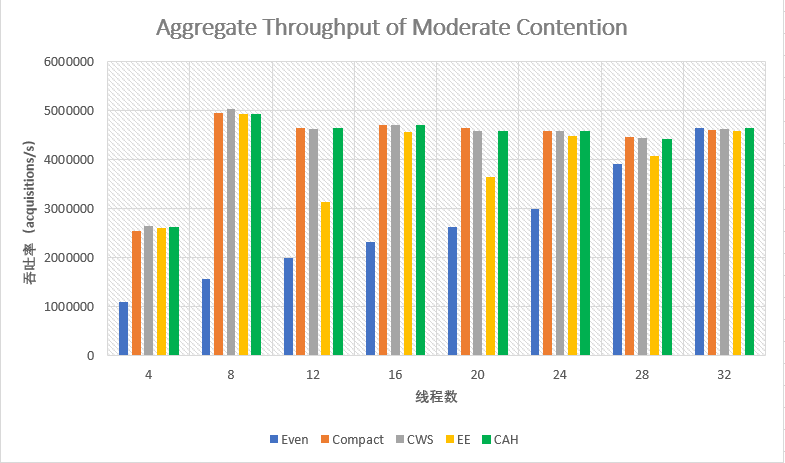
\includegraphics[width=5.6in]{throughput-moderate.PNG}
	\caption{竞争强度一般时吞吐率随线程数的变化}
	\label{Fig:throughput-moderate}
\end{figure}

\begin{figure}[t]
	\centering
	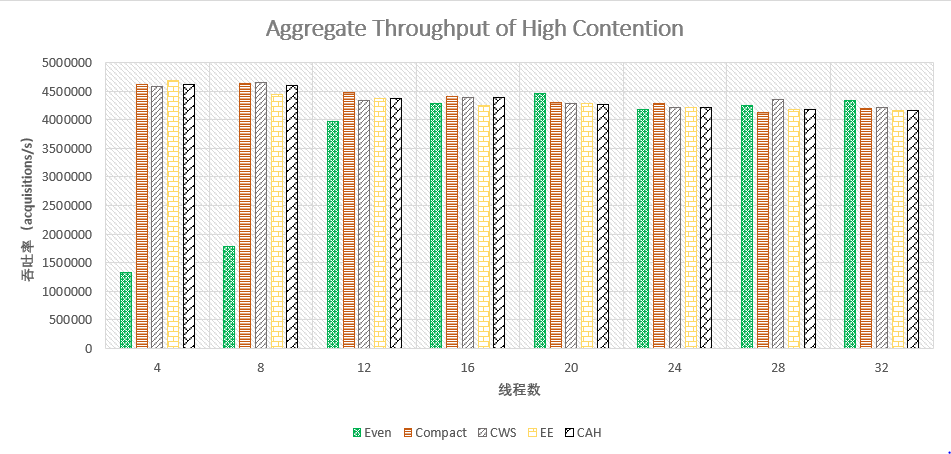
\includegraphics[width=5.6in]{throughput-high.PNG}
	\caption{高度竞争时吞吐率随线程数的变化}
	\label{Fig:throughput-high}
\end{figure}

\subsubsection{性能}
图\ref{Fig:throughput-moderate}和图\ref{Fig:throughput-high}分展示了stress\_one在C-MCS锁处于一般竞争强度(moderate contention,pause time 5000 cycle)和高度竞争(high contention,pause time 500 cycle)时,吞吐率在不同线程放置策略下随线程数的变化。从两图中可以看出:1)加强的平均放置(EE)相比平均放置(Even)性能有明显提升,这主要是因为EE在放置线程时使用了相对更少的NUMA节点,减少了锁的跨节点传递频率;2)有轮换的紧凑放置(CWS)与紧凑放置(Compact)的性能非常接近,这是因为我们的轮换策略是在线程空转等待锁的时候进行的,不会加长关键路径也就不会对性能产生明显影响;3)竞争感知的混合放置策略(CAH)的性能总是最高或者接近最高的,这说明CAH能保证总是获得接近最好的性能并且为了做竞争感知和混合放置而产生的额外代价没有对原有性能产生明显影响。另外,从图\ref{Fig:throughput-moderate}还可以看出竞争强度一般时,EE相比Compact或者CWS,其性能明显差很多,这是因为在竞争强度一般时,采用EE放置策略后可能所有节点上的本地MCS锁都没有饱和,而采用Compact或者CWS策略时,至少有一个节点上的本地MCS锁饱和,从而产生两者间的性能差异。


\subsubsection{长期公平性}

\begin{table}[!htbp]
  \centering
  \bicaption[竞争程度一般时的变异系数]
    {变异系数(moderate contention)}
    {Coefficient of Variation under Moderate Contention}
  \label{tab:CV-Moderate}
  \begin{tabular}{|c|c|c|c|c|c|}
    \hline
    \diagbox{线程数}{变异系数(\%)}{放置策略}&Even&Compact&CWS&EE&CAH\\
    \hline
    4	& 0.297282	& 0.066565	& 0.012887	& 0.013459	& 0.0128345 \\
    \hline
    8	& 0.106163	& 0.034858	& 0.009732	& 0.005521	& 0.034258 \\
    \hline
    12	& 0.022921	& {\bf 64.179479}	& 0.965768	& 1.252882	& 0.963768 \\
    \hline
    16	& 0.242998	& 1.331347	& 1.928579	& 0.443487	& 1.828579 \\
    \hline
    20	& 1.377443	& {\bf 46.017318}	& 0.908752	& {\bf \color{red}53.319157}	& 0.808752 \\
    \hline
    24	& 1.537792	& 0.941364	& 1.257626	& 1.296364	& 1.307626 \\
    \hline
    28	& {\bf \color{red}39.59038}	& {\bf 37.854002}	& 1.507482	& {\bf \color{red}37.392088}	& 1.007482 \\
    \hline
    32	& 0.981798	& 1.395845	& 0.622784	& 0.767253	& 0.722784 \\
    \hline
  \end{tabular}
\end{table}

\begin{table}[!htbp]
  \centering
  \bicaption[高度竞争时的变异系数]
    {变异系数(high contention)}
    {Coefficient of Variation under high Contention}
  \label{tab:CV-High}
 \begin{tabular}{|c|c|c|c|c|c|}
    \hline
    \diagbox{线程数}{变异系数(\%)}{放置策略}&Even&Compact&CWS&EE&CAH\\
    \hline
    4	& 0.493852	& 0.00039	& 0.002214	& 0.000510	& 0.00489 \\
        \hline
    8	& {\bf \color{red}7.292911}	& 0.002114	& 0.001629	& 0.001405	& 0.001229 \\
        \hline
    12	& {\bf \color{red}21.36302}	& {\bf 35.30975}	& 0.51774	& 0.019892	& 0.02774 \\
        \hline
    16	& 0.011835	& 0.006873	& 0.005782	& 0.005192	& 0.005682 \\
        \hline
    20	& 0.085078	& {\bf33.316092}	& 0.169483	& {\bf \color{red}7.267767}	& 0.767767 \\
        \hline
    24	& 0.005279	& 0.008571	& 0.010439	& 0.064837	& 0.094837 \\
        \hline
    28	& 0.019662	& {\bf 30.605009}	& 0.468846	& 0.064475	& 0.014475 \\
        \hline
    32	& 0.0089	& 0.02288	& 0.006184	& 0.004487	& 0.005487 \\
    \hline
  \end{tabular}
\end{table}

表\ref{tab:CV-Moderate}和表\ref{tab:CV-High}分别展示了stress\_one在C-MCS锁处于一般竞争强度(moderate contention)和高度竞争(high contention)时,单个线程吞吐率的变异系数在不同线程放置策略和不同线程数下的值。考虑到实验误差等因素的存在,我们认为变异系数小于2\%就是长期公平的。按照之前的建模分析,表中的五种线程放置策略中应该只有紧凑放置(Compact)会存在长期不公平的问题,但是从表\ref{tab:CV-Moderate}和表\ref{tab:CV-High}中可以看出在两种竞争强度下,Even和EE策略都存在表明长期不公平的异常数据,我们把所有表明长期不公平的数据进行了加粗标注,其中正常的数据用黑色加粗标注,异常数据用红色加粗标注,本小结我们暂时忽略这些异常数据,下一小节会对其进行详细分析。

不考虑异常数据的情况下,从表\ref{tab:CV-Moderate}和表\ref{tab:CV-High}中我们可以得出:1)紧凑放置(Compact)在某些情况下会导致严重的线程之间吞吐率的长期不公平,这是因为这些情况下Compact策略将线程分为了两个等价类;而其余情况下Compact没有造成长期不公平问题主要是因为这些情况下Compact与EE策略下最终的线程分布是相同的,即所有线程在一个等价类中;2)CWS在上述所有情况下都不会带来长期不公平的问题,对比Compact策略可以看出CWS通过使用线程轮换机制有效消除了不同等价类中的线程吞吐率差异。如图\ref{fig:high-12}所示,我们将其中一种情况的线程间吞吐率差异用劳伦茨曲线展示了出来,从这些曲线的“折线”特征可以看出线程之间的吞吐率差异主要体现在不同节点上的线程之间,对比Compact和CWS两种策略下的劳伦茨曲线可以看出轮换机制的有效性;3)CAH在上述所有情况下都避免了长期不公平的问题,虽然CAH本质上是EE和CWS的动态混合策略而EE存在长期不公平问题,但是CAH在EE存在长期不公平问题的情况下有效避免了采用EE策略,这主要是因为我们在策略选择是要求只有在每个节点上的平均线程数显著大于饱和点时才会采用EE策略,如公式\ref{Eq:policy}所示。


\begin{figure}[!htp]
  \centering
  \begin{subfigure}{8.0cm}
    \centering
    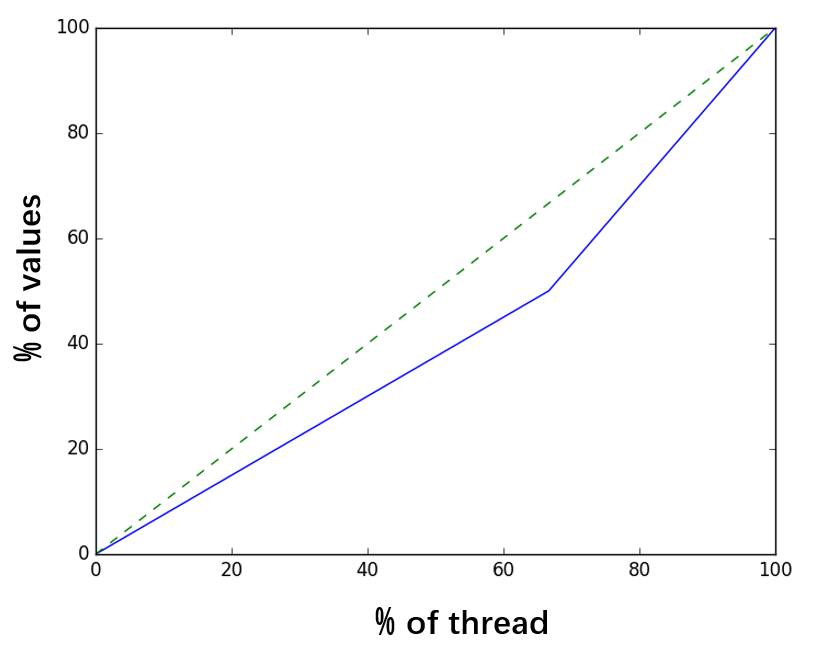
\includegraphics[height=5.5cm]{figure/compact-high-12.png}
    \caption{Lorenz Curve of Compact}
  \end{subfigure}
  \hspace{1em}
  \begin{subfigure}{6.0cm}
    \centering
    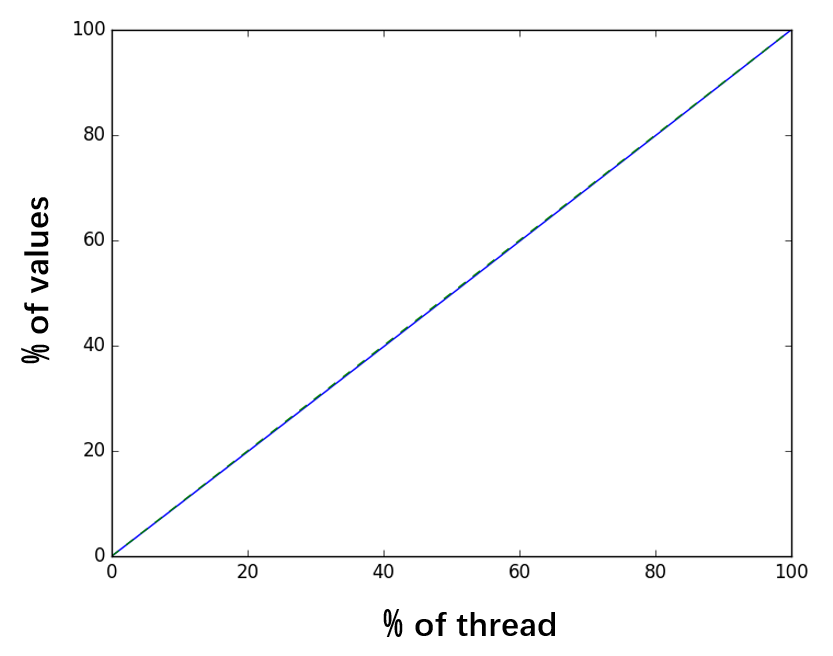
\includegraphics[height=5.5cm]{figure/CWS-high-12.PNG}
    \caption{Lorenz Curve of CWS}
  \end{subfigure}
  \bicaption{12threads,high contention,Lorenz Curve of Compact and CWS}{}
  \label{fig:high-12}
\end{figure}



\subsubsection{异常数据分析}

\begin{figure}[t]
	\centering
	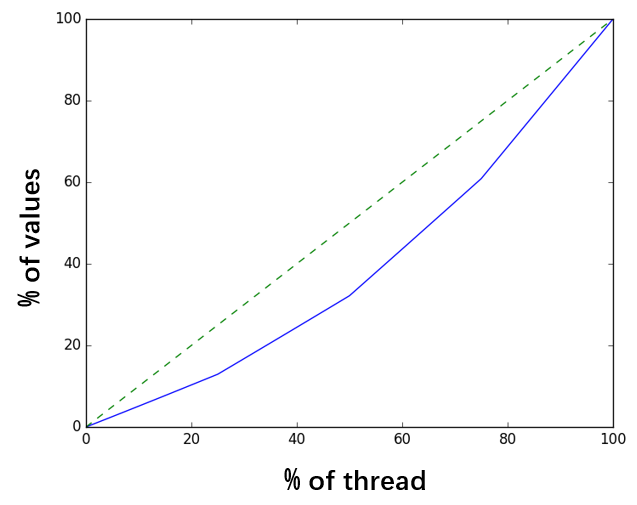
\includegraphics[height=5.5cm]{figure/Even-moderate-28.png}
	\caption{EE,moderate contention,28 threads,Lorenz Curve}
	\label{Fig:Even-moderate-28}
\end{figure}

对于表\ref{tab:CV-Moderate}和表\ref{tab:CV-High}出现的与之前建模和理论分析相违背的异常数据(红色加粗标注),我们猜想主要原因在于:1)出现异常的几个数据点对应的线程分布结果恰好满足每个节点上放置的线程数在锁当前的饱和点左右;2)不同NUMA节点上的核的性能存在差异,从而导致每个节点上的本地MCS锁的饱和点存在差异。上述两个原因导致的最终结果是虽然线程是平均分配到相关的节点上的,但是有些节点上的线程数恰好略大于对应的本地MCS锁饱和点,而有些节点上的线程数恰好略小于对应的本地锁的饱和点,从而最终的结果与Compact策略的结果类似。

上述猜想的理由有两点:
\begin{itemize}
    \item 我们以28个线程通过EE策略放置,在竞争一般的情况下为例,根据原始数据画出了28个线程之间吞吐率的劳伦茨曲线,如图\ref{Fig:Even-moderate-28}所示。该曲线具有明显的“折线”特征,并且由四道折线构成,对应28个线程分布在4个节点上。“折线”特征说明同一个节点上的线程的吞吐率没有显著差异,四个节点上放置的线程数相等(都是7个),理论上应该只有一道折线,上图中有四道折线说明这四个节点的计算性能存在差异。
    \item 对于图\ref{Fig:Even-moderate-28}对应的实验,我们只改变pause time然后观察变异系数的大小,得到图\ref{Fig:CV-pause}所示结果。随着pause time的减少,C-MCS锁当前的饱和点随着减小。当pause time小于6500 cycle时,所有节点上的本地锁都没有饱和,所以变异系数很小;当pause time介于6500 cycle和4500 cycle之间时,由于各个节点上核的性能差异,部分节点的本地MCS锁达到饱和,所以变异系数很大;而pause time小于4500 cycle时,所有节点上的本地MCS锁都得达到了饱和,所以变异系数接近0;
\end{itemize}

\begin{figure}[t]
	\centering
	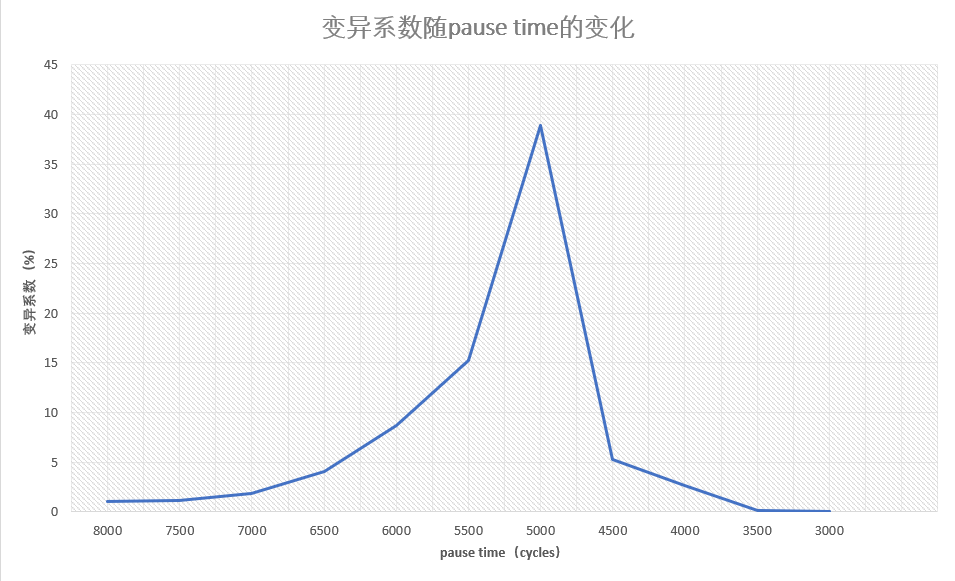
\includegraphics[width=5.6in]{figure/CV-pause.PNG}
	\caption{单个节点上的线程数处于饱和点附近时变异系数随pause time的变化}{}
	\label{Fig:CV-pause}
\end{figure}

\subsubsection{竞争动态变化}
\begin{table}[!hpb]
  \centering
  \bicaption[竞争动态变化时的不同策略对应的吞吐率]
    {竞争动态变化时的不同策略对应的吞吐率}
    {Throughput of Varying contention level}
  \label{tab:thrpt-varying}
  \begin{tabular}{@{}lllllr@{}} \toprule
    放置策略 & Even & Compact & CWS & EE & CAH\\ \midrule
    吞吐率(acquisitions/s)	&2433377	&4507560	& 4493016	& 4335519	& 4412345 \\
  \end{tabular}
\end{table}
在线程数为12,输入的pause time为5000 cycle时,我们在stress\_one内每200 ms 将pause time在500 cycle到5000cycle之间随机变化,然后统计总的吞吐率及单个线程的吞吐率分布。五种线程放置策略对应的吞吐率如表\ref{tab:thrpt-varying}所示。五种策略对应的单个线程的吞吐率的劳伦茨曲线如图\ref{fig:compact-even-varying}到图\ref{Fig:CAH-varying}所示。

Even策略吞吐率显著低于其他四种策略的吞吐率这是因为Even导致线程分布过于分散;Compact和CWS的吞吐率接近说明了shift机制对吞吐率影响比较小;CAH的吞吐率相比Compact和CWS有略微下降,原因应该是竞争感知和策略调整本身的所产生的代价;而EE策略相比Compact和CWS的吞吐率差异主要是竞争强度低时产生的。

从图\ref{fig:compact-even-varying}可以看出C-MCS锁中Even和Compact策略在竞争变化的情况下基尼系数(参考附录A)较大,存在较严重的长期不公平问题,其中Compact策略的不公平来源于线程的不均匀分布,而Even策略的不公平来源与不同节点核的计算能力差异(部分局部MCS饱和,如上节的异常数据分析)。从图\ref{fig:EE-CWS-varying}可以看出EE和CWS在本实验中大致可以保证长期公平性,其中CWS的公平性是通过额外的shift机制来保证的,而EE的公平性由线程的平均放置来保证。由于CAH基于CWS和EE机制实现,所以在本实验中在EE策略和CWS策略能保证长期公平性的前提下CAH框架自然也能保证长期公平性。

\begin{figure}[!htp]
  \centering
  \begin{subfigure}{8.0cm}
    \centering
    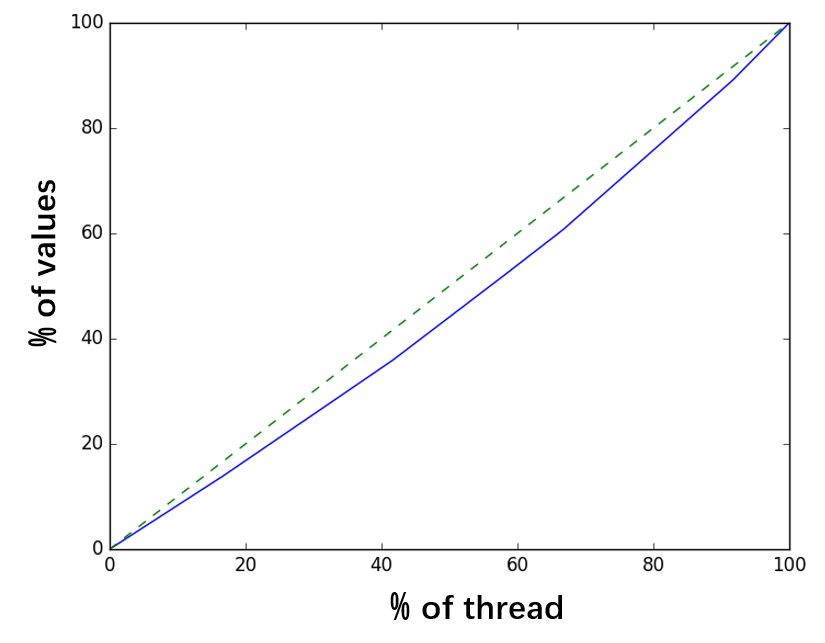
\includegraphics[height=5.5cm]{figure/even-varying.png}
    \caption{Lorenz Curve of Even}
  \end{subfigure}
  \hspace{1em}
  \begin{subfigure}{6.0cm}
    \centering
    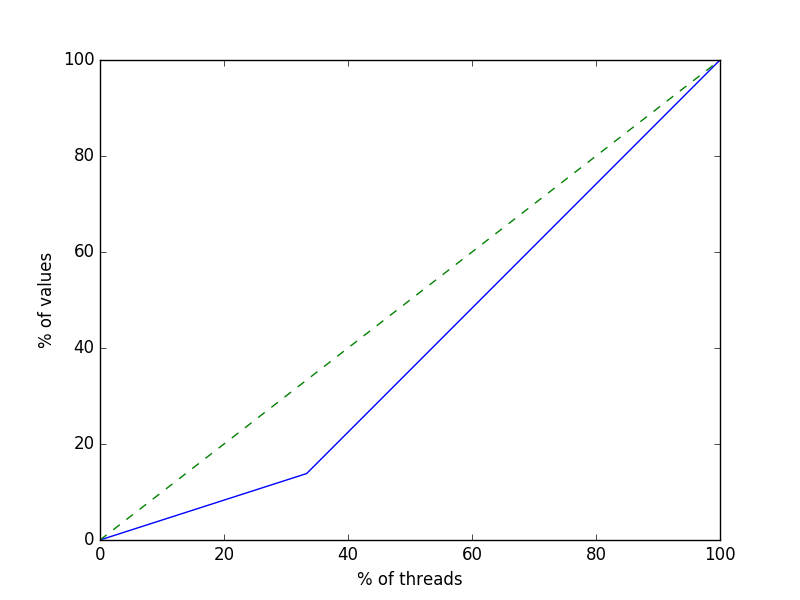
\includegraphics[height=5.5cm]{figure/compact-varying.png}
    \caption{Lorenz Curve of Compact}
  \end{subfigure}
  \bicaption{12threads,varying contention,Lorenz Curve of Even and Compact}{}
  \label{fig:compact-even-varying}
\end{figure}


\begin{figure}[!htp]
  \centering
  \begin{subfigure}{8.0cm}
    \centering
    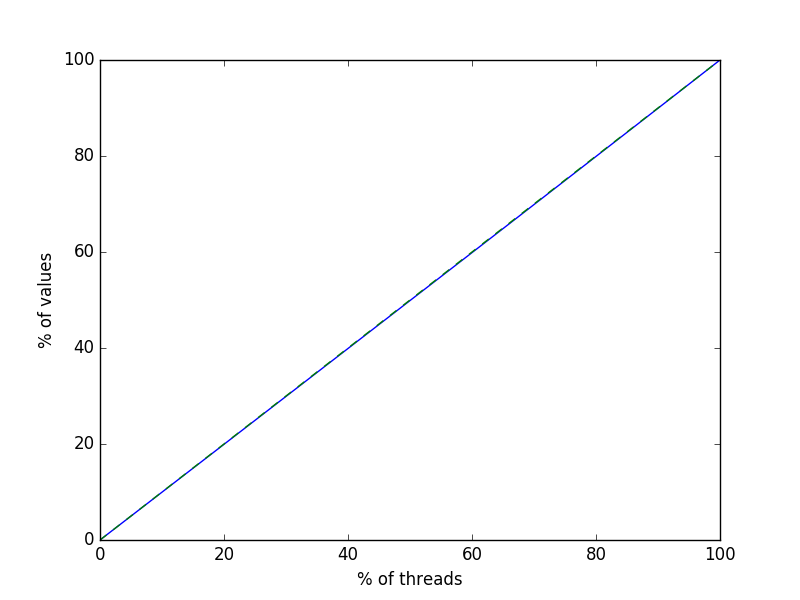
\includegraphics[height=5.5cm]{figure/EE-varying.png}
    \caption{Lorenz Curve of EE}
  \end{subfigure}
  \hspace{1em}
  \begin{subfigure}{6.0cm}
    \centering
    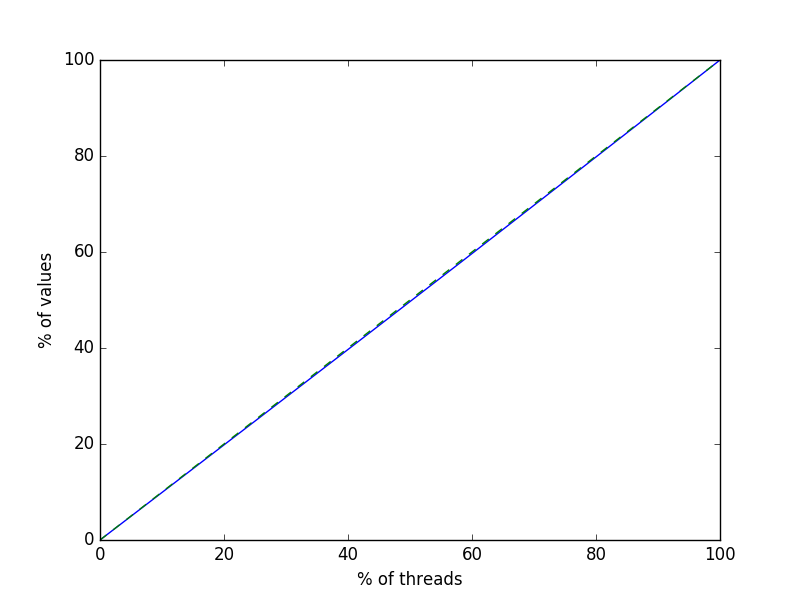
\includegraphics[height=5.5cm]{figure/CWS-varing.png}
    \caption{Lorenz Curve of CWS}
  \end{subfigure}
  \bicaption{12threads,varying contention,Lorenz Curve of EE and CWS}{}
  \label{fig:EE-CWS-varying}
\end{figure}

\begin{figure}[t]
	\centering
	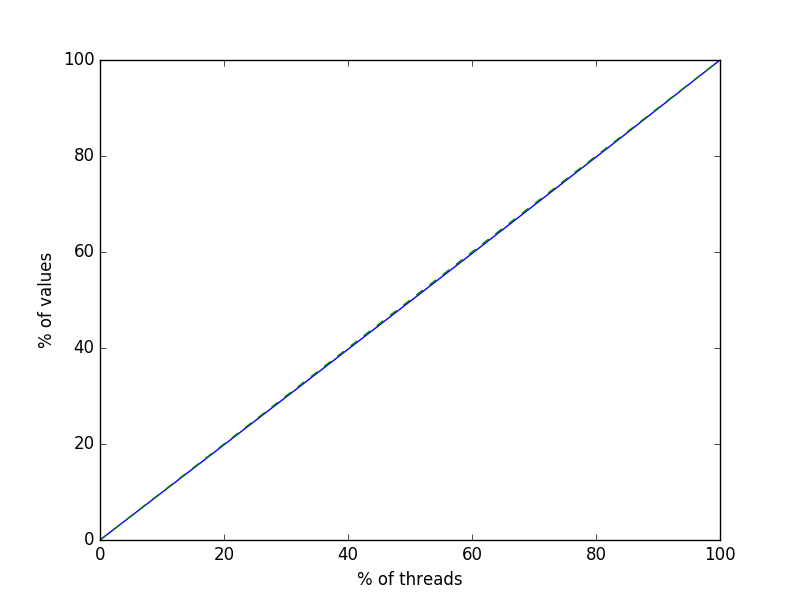
\includegraphics[height=5.5cm]{figure/CAH-varying.png}
	\caption{Lorenz Curve of CAH, 12threads,varying contention,Lorenz Curve of CAH}{}
	\label{Fig:CAH-varying}
\end{figure}

\subsection{Memcached实验}
\subsubsection{Memcached}
Memcached是一个广泛使用的开源、高性能、分布式内存key-value data store,它通常被用来作为高性能应用的数据库的缓存层来使用。包括Facebook、LiveJournal、Wikipedia、Flickr、YouTube、Twitter等在内的很多知名产品中都有用到Memcached。

在Memcached中,所有的键值对都存在一个巨大的哈希表中,所有服务端的线程并行访问该哈希表。该哈希表包含了大量的桶(bucket),每个bucket由一个细力度的锁来做访问控制,另外有一个叫做cache\_lock的全局锁(global lock,不同于层级锁中的全局锁)来保护整个哈希表。在做维护(maintenance)和再平衡(rebalance)等操作的时候会使用到该全局锁。cache\_lock是Memcached中公认的竞争瓶颈\cite{pohlack2011lightweight},所以Memcached很适合用来作为本文的测试benchmark。Memcached中该cache\_lock是用Pthread mutex实现的,我们使用LiTL库在运行时将其替换为了采用LiTL统一接口重写的C-MCS锁。

Memcached API包含了两个对key-value的基本操作:get(返回给定键对应的值)和set(更新给定键对应的值),其中这两个操作对cache\_lock的影响如下:get操作只会用到bucket对应的细力度锁,不会用到cache\_lock,也就是说不会造成cache\_lock的竞争,所以我们后续实验对Memcached 的测试不会用到get操作;set操作会造成对cache\_lock的大量竞争,进而对Memcached的性能和其他特性造成影响,所以我们后续实验将只使用set来测试Memcached。现实应用中get操作是Memcached服务器中占绝大多数的操作,但是也有些场景下set操作占绝大比例,比如收集大量的传感器网路的数据、持续更新大量条目的数据信息等\cite{dice2012lock}。

为了生成对Memcached服务器的负载,我们使用了memslap,一个针对Memcached的负载产生和测试工具。memaslap是Memcached的标准客户库(叫做libMemcached\cite{libmemcached})的一部分。我们通过控制memslap客户端的并发线程数来调节Memcached中cache\_lock的竞争程度,实验中memaslap 和 Memcached分别运行在两台相同的Intel Xeon E5机器上。另外测试结束后memaslap 和 Memcached都只会报告总的吞吐率数据,为了计算变异系数、绘制劳伦茨曲线等进而衡量长期公平性,我们必须知道每个线程的吞吐率。为了得到每个线程的吞吐率,我们在C-MCS锁中放锁的时候由每个线程统计自身的吞吐率,然后为SIGUSR1信号注册了一个处理函数,在该处理函数中输出每个线程的吞吐率及变异系数等其他统计信息,测试运行结束后只需要向Memcached服务器发送SIGUSR1信号就可以得到上述信息,如下代码所示:
\begin{lstlisting}[language={Bash}, caption={获取Memcached每个线程的吞吐率及其他统计信息}]
ps -aux | grep "memcached"
kill -s SIGUSR1 <pid>
\end{lstlisting}
其中pid是Memcached服务器的进程号。

在本实验中,我们将memcached服务端线程数固定为12,因为这种情况下各个线程放置策略生成的最终线程分布差异较大。我们将客户端memslap的并发数设置为服务端线程数的整数倍,我们在前期实验中发现memcached服务端按照Round-Robin的方式调度服务端线程处理客户端请求,客户端的同一个socket流的请求在一定时间内是由同一个服务端线程处理的,所以将客户端的并发数设置为服务端线程数的整数倍可以避免memcached对客户端请求的调度造成的对cache\_lock的长期公平性的统计误差。
\subsubsection{性能}

\begin{figure}[t]
	\centering
	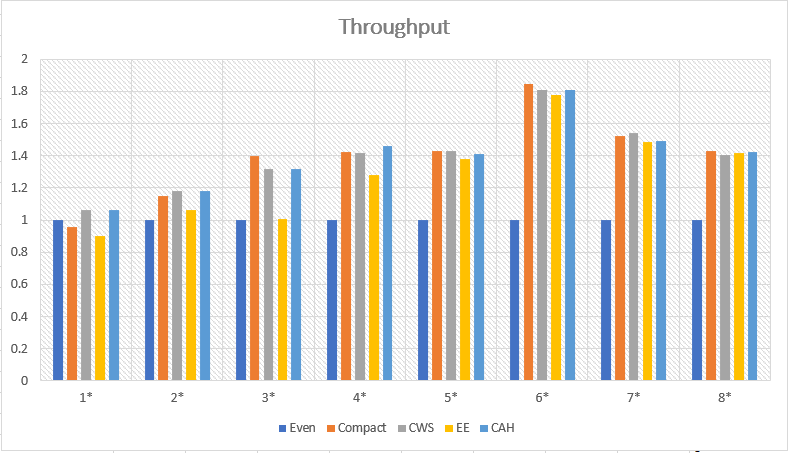
\includegraphics[width=5.6in]{figure/memcached-throughput.PNG}
	\caption{memcached中不同负载下五种线程放置策略对应的吞吐率差异}{}
	\label{Fig:memcached-thrpt}
\end{figure}
如图\ref{Fig:memcached-thrpt}所示,memcached服务端运行有12个线程,客户端memslap的并发数是12的整数倍,我们依次测了memslap端的并发数是12的一到八倍时各种线程放置策略对应的吞吐率差异,并以Even策略的吞吐率为基础,对其他策略的吞吐率做了归一化处理。第一组数据中Compact和EE策略的吞吐率略低于Even策略的吞吐率的主要原因应该是负载太小,各种策略对吞吐率的影响并不明显。在负载足够大的情况下,Compact策略的吞吐率总是最高或者接近最高的,这说明了在负载充分大时,数据访问的局部性对于性能的影响比较显著。CWS的吞吐率相比Compact并没有明显差距,这说明在memcached中额外的轮换操作也没有带来性能的明显损失。负载较大时EE策略相比Even策略的吞吐率有较大提升说明跨节点的锁传递频率是竞争激烈时影响性能的关键因素。 EE策略相比Compact和CWS的吞吐率差异随着负载的增加而逐渐减小,这是因为负载的增加导致服务端线程请求锁的频率增加,弥补了EE策略本身不能充分挖掘局部性的不足。memcached实验中各种放置策略对总的吞吐率的影响与stress\_one实验结果的趋势大致相同。但是具体来看每个线程的吞吐率上的话,同一个节点上的线程之间会有较大的吞吐率差异,表现在劳伦茨曲线上就是该曲线不再具有明显的“折线”特征,这主要是因为Memcached本身对客户端的请求的调度并不是绝对公平的。
\subsubsection{长期公平性}
\begin{figure}[t]
	\centering
	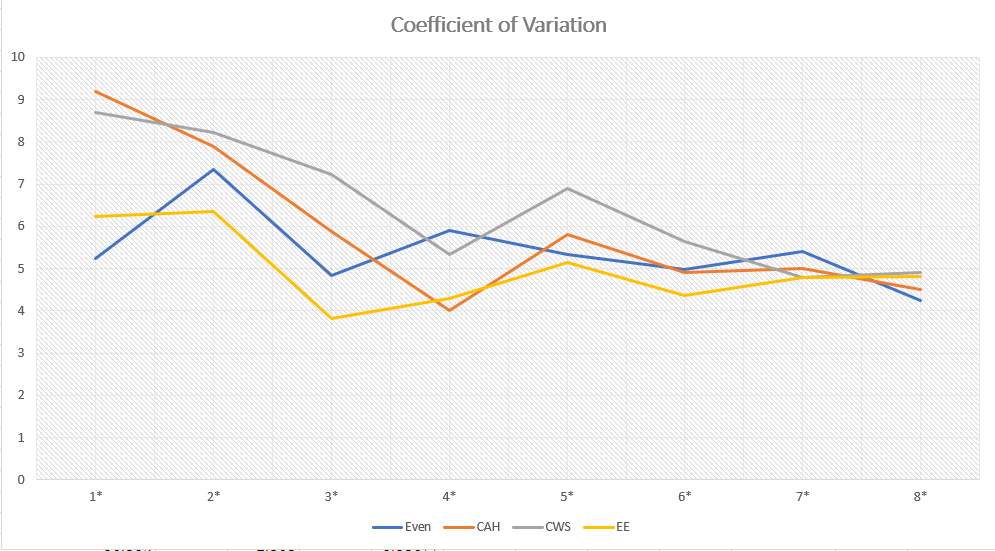
\includegraphics[width=5.6in]{figure/memcached-cv.PNG}
	\caption{memcached中不同线程放置策略对应的变异系数与负载关系}{}
	\label{Fig:memcached-fairness}
\end{figure}


图\ref{Fig:memcached-fairness}显示了除Compact策略以外的其他线程放置策略在不同负载强度下对memcached服务端线程吞吐率的变异系数即长期公平性的影响;表\ref{tab:CV-Compact}显示了Compact策略在不同负载强度下对应的单个线程吞吐率的变异系数。总得来看,除了Compact策略以外,其他策略中随着负载的增加变异系数呈下降趋势,这是因为负载越大,锁对memcached服务端线程的行为影响越明显,总的统计数据也就与之前的理论分析越吻合。EE策略和Even策略在理论上能够保证长期公平性,其对应的变异系数的稳定值理论上应该接近于0,而图\ref{Fig:memcached-thrpt}中该值在5\%左右,说明memcached本身的负载调度和其他因素的对于线程间的吞吐率差异的影响较稳定,表现在变异系数上就是5\%左右。对比CWS和Compact策略可以看出CWS的轮换机制能够显著抹平由于紧凑放置而导致的线程之间吞吐率的巨大差异,极大地改善长期公平性。而CAH框架对应的变异系数稳定地趋近于EE和CWS的变异系数,说明CAH能够在各种负载/竞争状况下保持较好的长期公平性。
\begin{table}[H]
  \centering
  \bicaption[Compact策略的变异系数]
    {12个线程时Compact策略的变异系数}
    {Coefficient of Variation under Compact Strategy}
  \label{tab:CV-Compact}
  \begin{tabular}{@{}llllllllr@{}} \toprule
    负载 & 1* & 2* & 3* & 4* & 5* & 6* & 7* & 8*\\ \midrule
    变异系数(\%)	&10.43	&29.8	& 30.7	& 42.6	& 52.3 &50.3 &42.8 &40.6 \\
  \end{tabular}
\end{table}
\section{本章小结}
本章通过在stress\_one和memcached两个benchmark上的实验比较了五种线程放置策略对C-MCS锁的性能和长期公平性的影响,实验结果说明EE策略相比原有的Even策略能在负载较大竞争较激烈时获得更好的性能;CWS策略相比Compact策略能在没有明显性能损失的前提下保证长期公平性;而CAH框架能以尽可能小的额外代价在包括负载/竞争强度变化的情况下获得接近最好的性能和可靠的长期公平性。